\chapter{Time Series}
\label{ch:time-series}

In previous chapters, we have always analyzed data collected at a specific moment in time and we made statements about that data for that specific moment.

However, within the context of IT, it might be required to monitor data that is constantly changing. For example, think of the load on a processor, the evolution of disk usage on a storage device, the response time of a website, etc.

In this chapter we will examine this type of data and discuss the main analysis methods.

\section{Learning Goals}
\label{sec:time-series-learning-goals}

By the end of this chapter you must be able to:

\begin{itemize}
  \item Explain the following concepts:
  \begin{itemize}
    \item Time series, moving average
  \end{itemize}
  \item For a given time series, i.e. a series of observations from a time series:
  \begin{itemize}
    \item Apply the moving average method;
    \item Based on a plot of observations, estimate what type of exponential smoothing (basic, double, triple/Holt-Winters) is best suited;
    \item Predict future values;
  \end{itemize}
  \item Understand and explain the formulas for the moving average and exponential smoothing, in particular, to estimate the effect of the value of parameters; 
\end{itemize}

  \section{Time Series \& Predictions}

  \begin{definition}[Time Series]
    A \emph{time series} is a sequence of observations of an arbitrary variable in time order.
\end{definition}

Examples:

\begin{itemize}
	\item monthly demand for milk
	\item annual intake of students at HOGENT
	\item daily flow rate of a river
	\item the outside temperature over the course of a day
\end{itemize}

Predicting time series is an important part of research because they often form the basis for decision models. Examples include:

\begin{itemize}
	\item general development of future plans (investments, capacity \dots)
	\item budget planning to avoid shortcomings (operating budget, marketing budget \dots)
	\item competitive delivery times of a company
	\item support for financial objectives
	\item avoid uncertainty
	\item the possibility to quantitatively model developments in road safety
\end{itemize}


Modeling time series is a statistical problem: we assume that the observations vary according to a certain probability density function as a function of time. We often assume that the observations in a time series are correlated and therefore are not obtained from a random sample.

Different model types are used to analyze time series. These models have in common that in principle they can not only describe the development in an observed time series, but they can also be used to

\begin{itemize}
	\item find explanations for this development and
	\item to predict the future values of the time series.
\end{itemize}

However, their suitability for achieving these objectives varies widely. In this chapter we limit ourselves to using time series with a history to determine time dependent models. An example of a time series is the age of the successive kings of England starting from William The Conqueror \autocite{Hipel1994}.

\begin{lstlisting}
kings <- scan(file = 'syllabus/data/time-series/kings.data', skip = 3)
kingstimeseries <- ts(kings)
plot.ts(kingstimeseries, ylab='age', xlab="time")
grid(lty=2,lwd=1,col='black')
\end{lstlisting}

\begin{figure}
	\centering
	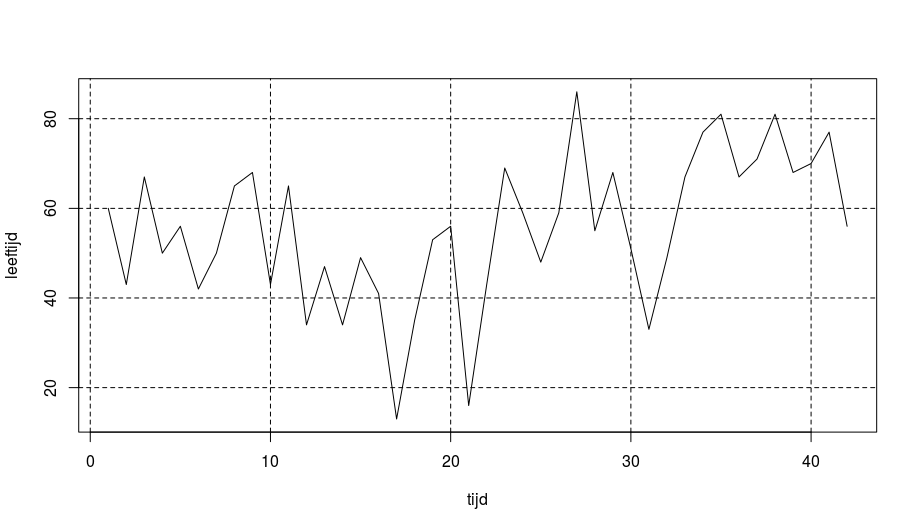
\includegraphics[width=\textwidth]{time-series/time-series-kings.png}
	\caption{The time series representing the ages of the kings.}
	\label{fig:time-series-11}
\end{figure}

\section{Time series models}

\subsection{Mathematical model}

Our goal is to create a model that explains the observed data and that allows to predict future observations as accurately as possible. The simplest model you can think of is a model where a constant $b$ is used with variations around $b$ determined by a random variable $\epsilon_{t}$ as in Equation~\ref{eq:constant}.

\begin{equation}
	X_{t} = b + \epsilon_{t}
\label{eq:constant}
\end{equation}

\begin{description}
  \item [$X_{t}$] represents a \emph{variable} that is unknown at time $t$.
  \item [$x_{t}$] represents an \emph{observation} at time $t$ (and is known). 
  \item [$\epsilon_{t}$] is called the \emph{noise} and is considered to have a mean of $0$ with variance $\sigma^{2}$ and has a normal distrbution ($\epsilon_{t} \sim Nor(0, \sigma)$). 
\end{description}

We could also assume that there is a linear relationship:

\begin{equation}
  X_{t} = b_{0} + b_{1} \times t + \epsilon_{t}
  \label{eq:linear8}
\end{equation}

The equation in \ref{eq:constant} and \ref{eq:linear8} are special cases of the polynomial case:

\begin{equation}
	X_{t} = b_{0} + b_{1} t + b_{2} t^{2} + \dots + b_{n} t^{n} + \epsilon_{t} 
\label{eq:polynomial}
\end{equation}

\begin{exercise}
	What could the following time series represent?
	\begin{equation}
		X_{t} = b_{0} + b_{1} \sin\left(\frac{2\pi t}{4}\right) + b_{1} \cos\left(\frac{2\pi t}{4}\right) + \epsilon_{t}
	\label{eq:seasonal}
\end{equation}
\end{exercise}

Answer: This is a cyclic time series with period $= 4$. This could for example be used with a time series for seasons.

\begin{lstlisting}
f <- function(a, b,t){
  return(a + b * sin((2 * pi*4)/4) + b * cos((2 * pi*4)/4) + rnorm(1))
}
t <- seq(from = 1, to = 100, by = 1)
X <- lapply(t,f,a=5,b=5)
plot(x = t, y=X, type = 'l')
\end{lstlisting}

\subsubsection{General}

In each considered model, the time series is a function of time and parameters of the model. In general, we can say that:

\begin{equation}
	X_{t} = f(b_{0}, b_{1}, b_{2}, \dots , b_{t}, t) + \epsilon_{t}
\label{eq:general}
\end{equation}

We then accept the following statements:

\begin{itemize}
	\item The model assumes two components of variability: the mean of the predictions changes with time and the variations to this mean vary randomly.
	\item The residuals of the model ($X_{t} - x_{t}$) are homoscedastic: this means that they have a constant variance in time.
\end{itemize}

Once the model is chosen, all that remains is the problem of estimating the parameters for Equation~\ref{eq:general}. This will be discussed in the following sections.

\section{Estimating the parameters}

Once a model is selected, it is up to the researcher to estimate the parameters, i.e. find parameters that ensure that the model approximates the observed values as closely as possible. We usually assume that all values are equivalent, but this is not the case with time series. Since our independent parameter is time, we need to obtain methods that make more recent data more important than old data or vice versa.

In what follows we describe the time series with estimated values for the parameters. We indicate estimators by using a hat on the parameters:

\[ \widehat{b}_{1}, \widehat{b}_{2} \dots \widehat{b}_{n} \]

\subsection{Moving average}

\begin{table}
  \centering
  \begin{tabular}{|l|l|l|l|l|l|l|l|l|l|}
    \hline
    4 & 16 & 12 & 25 & 13 & 12 & 4 & 8  & 9 & 14 \\ \hline
    3 & 14 & 14 & 20 & 7  & 9  & 6 & 11 & 3 & 11 \\ \hline
    8 & 7  & 2  & 8  & 8  & 10 & 7 & 16 & 9 & 4  \\ \hline
  \end{tabular}
  \caption{Time series data example, visualized in Figure~\ref{fig:time-series-21}.}
  \label{tab:data-time-series-21}
\end{table}

Suppose a researcher has the data of Table~\ref{tab:data-time-series-21} up to the twentieth point available (known data). The researcher does not know the subsequent data points and has to predict them. A first model that could be used is the constant model from Equation~\ref{eq:constant}.

According to this model, the data points are considered as random values from a population with a mean $b$. The best estimator for $b$ is the mean of these twenty data points.

\begin{lstlisting}
data <- c(4 , 16 , 12 , 25 , 13 , 12 , 4 , 8  , 9 , 14, 
+           3 , 14 , 14 , 20 , 7  , 9  , 6 , 11 , 3 , 11, 
+           8 , 7  , 2  , 8  , 8  , 10 , 7 , 16 , 9 , 4 )
mean(data[1:20])
\end{lstlisting}

\[ \widehat{b} = \frac{1}{20} \sum_{1}^{20} x_{t}= 10.75 \]

This is the best estimator based on the 20 data points. However, note that $x_{1} =  4$ has as much \textit{value} as  $x_{20} = 11$, or in other words: the coefficient of $x_{1}$ is the same as the coefficient of $ x_ {20} $, which is $\frac{1}{20}$.

If we use this as an estimator, Figure~\ref{fig:time-series-21} illustrates that this is not a good idea.

\begin{lstlisting}
AV20 <- matrix(10.75,30,1)
plot.ts(data, col="blue", type='b', xlab='time', ylab='Data')
lines(AV20,col='red', type='l')
legend(x= 'topright',legend = c("Data","Mean 10.75"), lty = c(1,1), lwd = c(2.5,2.5), col=c('blue','red'))
\end{lstlisting}

\begin{figure}
	\centering
		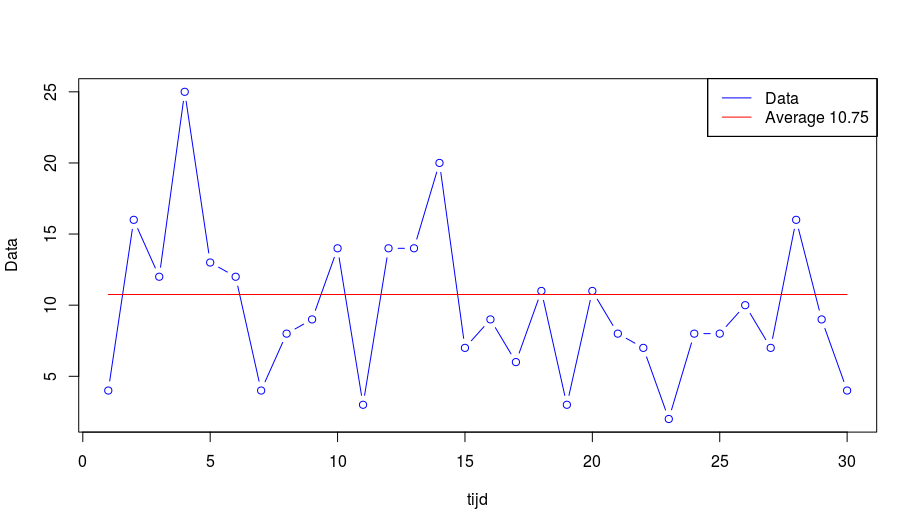
\includegraphics[width=1.00\textwidth]{time-series/time-series-20.png}
	\caption{Time series with constant mean $10.75$}
	\label{fig:time-series-21}
\end{figure}

If we assume that the data changes over time, it is better to have old data count less than more recent ones. One possibility is to use only recent data, for example the 10 or 5 last data points (cfr. Figure \ref{fig:time-series-31}).

\[ \widehat{b} = \frac{1}{10} \sum_{10}^{20} x_{t} = 10.18 \] and
\[ \widehat{b} = \frac{1}{5} \sum_{15}^{20} x_{t} = 7.83 \]

\begin{lstlisting}
sma10 <- SMA(x =data,n=10)
sma5 <- SMA(x=data,n=5)
plot.ts(x = data, col = 'blue',type = 'l')
lines(sma10, col='red', type = 'b')
lines(sma5, col='purple', type = 'b')
\end{lstlisting}

\begin{figure}
  \centering
    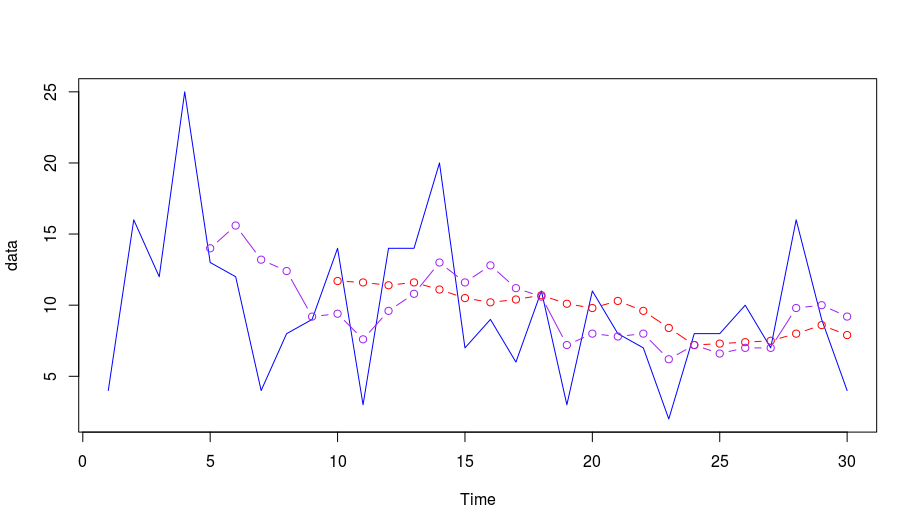
\includegraphics[width=1.00\textwidth]{time-series/time-series-sma.png}
    \caption{Time series with moving average $m = 10$ and $m=5$}. 
  \label{fig:time-series-31}
\end{figure}

These are called \textit{moving averages}\index{moving average}.

Which estimator is now best? We cannot answer this yet.

\begin{itemize}
  \item The estimator using all data points is best if the time series follows the model completely.
  \item The estimator with the more recent data points is best if the time series changes over time.
\end{itemize}

\begin{definition}[moving average]
  In general the \emph{moving average} is the average (mean) of the last $m$ observations.
  \begin{equation}
    \widehat{b} = \sum_{i=k}^{t} \frac{x_{i}}{m}
  \label{eq:movingAverage}
  \end{equation}
  with $k = t-m+1$. $m$ is the time range and is the parameter of the method.
\end{definition}

\subsection{Measuring the accuracy of predictions}

%\begin{table}
%  \centering
%\begin{tabular}{|lllllllllll|}
%
%\end{tabular}
%\caption{Voorspellingsfout voor een moving average $m = 10$}
%\label{tab:error}
%\end{table}

One method for measuring the prediction is calculating the mean absolute deviation ($MAD$): the mean of the absolute differences between the predicted and actual values of the time series.

\begin{definition}[$MAD$]
  \begin{equation}
    MAD = \frac{1}{n} \sum_{1}^{n} \left| e_{i} \right|  
  \label{eq:MAD}
  \end{equation}
\end{definition}

You can also percentage this to calculate the mean absolute percentage error ($MAPE$), also known as mean absolute percentage deviation ($MAPD$).

\begin{definition}[$MAPE$]
  \begin{equation}
    MAPE = \frac{1}{n} \sum_{1}^{n} \left| \frac{e_{i}}{X_i} \right|  
  \label{eq:MAD2}
  \end{equation}
\end{definition}

It is also possible to calculate the variance of the errors:

\begin{definition}[$VAR$]
\begin{equation}
	s^{2}_{e} = \frac{1}{m} \sum_{1}^{n} (e_{i} - \overline{e})^{2}
\label{eq:varError}
\end{equation}
\end{definition}

% TODO: moet de noemer hierboven niet n - 1 zijn??

A last insteresting parameter is the root-mean-square error ($RMSE$) or root-mean-square deviation ($RMSD$), which is the square root of the mean of the squared difference between the predicted and the actual values of the time series.

\begin{definition}[$RMSE$]
  \begin{equation}
    RMSE_{e} = \sqrt{\frac{1}{m} \sum_{1}^{n} (e_{i})^{2}}
  \label{eq:varError2}
  \end{equation}
\end{definition}

\section{Exponential smoothing}

When calculating a moving average, all previous observations have equal weight. With exponential smoothing, however, smaller weights are assigned to older observations. In other words, more recent observations gain relatively more weight than older observations.

In the case of the simple moving average, all weights are the same, namely $\frac{1}{m}$.

\subsection{Basic exponential smoothing}

Exponential smoothing is a weighted arithmetic mean that assigns positive weights to the current and past values of a time series. A single weight, $0\leq \alpha \leq1$ or the smoothing constant is selected for this. For a given time $t$, the basic exponential smoothing can be found using Equation \ref{eq:singleExpSmooting}.

\begin{definition}[Exponential Smoothing]
  \begin{equation}
    X_{t} = \alpha x_{t} + (1-\alpha)X_{t-1}, 0 \leq \alpha \leq 1, t \geq 3
  \label{eq:singleExpSmooting}
  \end{equation}
\end{definition}

In other words, $X_{t}$ is a weighted arithmetic mean of the current observation $x_t$ and the previous exponential smoothing $X_{t-1}$.

\subsection{Initial value}
Determining $X_{2}$ is an important parameter. You could choose to:
\begin{enumerate}
  \item assume that $X_{2} = x_{1}$
  \item make $X_{2}$ equal to a specific objective
  \item take the mean of the first $x$ observations
  \item \dots
\end{enumerate}

Why is this called an exponential method? If we were to substitute we find e.g. for $X_{t-1}$:

\[ X_{t} = \alpha x_{t} + (1-\alpha)\left[\alpha x_{t-1} + (1-\alpha)X_{t-2}\right] \] 
\[ X_{t} = \alpha x_{t} + \alpha (1-\alpha)x_{t-1} + (1-\alpha)^{2} X_{t-2} \]
or in general:
\[ X_{t} = \alpha \sum_{i=0}^{t-2}(1-\alpha)^{i-1}x_{t-i} + (1-\alpha)^{t-2} X_{2}, t \geq 2 \]

You will notice that older components have an exponentially smaller weight.

\subsubsection{Value of $\alpha$}
The speed at which the old observations are ``forgotten'' depends on the value of $\alpha$. For a value of $\alpha$ close to 1, old observations are quickly forgotten , whereas for  $\alpha$ close to 0, this goes less fast (as illustrated in Table \ref{tab:alpha}). Often a value between $0.10$ and $0.30$ is used.

\begin{table}
  \centering
  \begin{tabular}{l|llll}
  $\alpha$ & $(1-\alpha)$ & $(1-\alpha)^{2}$ & $(1-\alpha)^{3}$ & $(1-\alpha)^{4}$ \\ \hline
  0.9   & 0.1       & 0.01             & 0.001                      & 0.0001           \\
  0.5   & 0.5       & 0.25             & 0.125                      & 0.062            \\
  0.1   & 0.9       & 0.81             & 0.729                      & 0.6561           \\
  \end{tabular}
  \caption{Values for $\alpha$ and $(1-\alpha)^{n}$}
  \label{tab:alpha}
  \end{table}

  For example, the file \texttt{precip.data} contains the total annual rainfall in inches for London, between 1813 and 1912. Let's analyse this in R.
  
\begin{lstlisting}
rain <- scan("cursus/data/tijdreeksen/precip.data",skip=1)
rainseries <- ts(rain,start=c(1813))
plot.ts(rainseries)
plot(rainseriesforecasts)
\end{lstlisting} 

%TODO figuur maken voor verschillende alpha's

\subsubsection{Prediction with exponential smoothing}

Suppose the goal is to predict the next value $X_{t+1}$, this is equal to calculating the the smoothing value at time $t$.

\begin{equation}
	X_{t+1} = EMA_t = X_t
	\label{eq:EMA}
\end{equation}

With $X_t$ the last predicted value.

This can be easily done in R. The outcome is a \emph{prediction interval}, an interval for which we expect the predicted value to be included with a certain probability. By default, an 80\% and a 95\% interval are returned.

\begin{lstlisting} 
library('forecast')
rainseriesforecasts2 <- forecast.HoltWinters(rainseriesforecasts, h=8)
plot.forecast(rainseriesforecasts2)
\end{lstlisting} 

We should see correlations between the prediction errors for subsequent predictions. In other words, if there is a correlation between forecast errors for subsequent predictions, it is more likely that the simple exponential smoothing can be corrected by using a different prediction technique.

To find out if this is the case, we can obtain a correlogram of the in-sample prediction errors.

We remembers from Chapter~\ref{ch:bivariate-analysis} that the covariance or correlation describe the relationship between two variables. The autocovariance and autocorrelation measure the linear relationship between time-shifted values for a time series.

\begin{definition}[Autocovariance]
  We define the autocovariance for a lag $k$ as $c_k$.
	\[ c_k = \sum_{t=k+1}^{T} (y_t - \overline{y})(y_{t-k} - \overline{y}) \]
\end{definition}

\begin{definition}[Autocorrelation]
  We define the autocorrelation for a lag $k$ as $r_k$.
	\[ r_k = \frac{c_k}{c_0} \]
\end{definition}

A correlogram is a plot of the autocorrelations. You can plot this in R by using the function \texttt{acf()}. This also calculates the prediction errors. To determine the maximum lag (delay) we want to view, we use the parameter \texttt{lag.max}.

For example, to calculate a correlogram of the forecast errors for the London rainfall data for a lag between 1 and 20, we use:

\begin{lstlisting}
acf(rainseriesforecasts2$residuals, lag.max=20, na.action = na.pass)
\end{lstlisting}

To test whether there is significant evidence for significant correlations at a lag 1-20, we can apply a Ljung-Box test. This can be done in R using the function \texttt{Box.test()}. The maximal lag (or delay) we want to investiage, is specified using the parameter \texttt{Lag}.

A full explanation of this test is out of scope for this course, but the test assumes the hypotheses $H_0$ and $H_1$ as formulated below. The tes statistics can then be interpreted in a similar way as all other  hypothesis tests described in the previous chapters.

\begin{itemize}
  \item $H_0$ The data are independently distributed (in other words, the correlations in the population from which the sample is taken are 0, and therefore  any observed correlations in the data result from randomness of the sampling process).
  \item $H_1$ The data are not independently distributed, they exhibit linear (serial) correlation.
\end{itemize}

For example, to test that there are no zero autocorrelations for a lag 1-20, for the in-sample predictions errors for London rainfall data, we type:

% TODO: correcte Nl term voor in-sample error?

\begin{lstlisting}
Box.test(rainseriesforecasts2$residuals, lag=20, type="Ljung-Box")
Box-Ljung test
data:  rainseriesforecasts2$residuals
X-squared = 17.4008, df = 20, p-value = 0.6268
\end{lstlisting}

Finally, we should also look at the distribution of the errors of the forecast. As mentioned above, we assume that the errors are normally distributed with an average $\mu = 0$ and a constant standard deviation. To verify this assumption, we can plot a histogram of the forecast errors, with an overlapping normal curve with mean zero and the same standard deviation as the distribution of the prediction errors. For this, we can define a function in R \texttt{plotForecastErrors()}. It is also recommended to use the methods described in Section~\ref{ssec:testing-for-normality}.

% TODO: zin onvolledig

\begin{lstlisting}
plotForecastErrors <- function(forecasterrors)
{
# make a histogram of the forecast errors:
mybinsize <- IQR(forecasterrors)/4
mysd   <- sd(forecasterrors)
mymin  <- min(forecasterrors) - mysd*5
mymax  <- max(forecasterrors) + mysd*3
# generate normally distributed data with mean 0 and standard deviation mysd
mynorm <- rnorm(10000, mean=0, sd=mysd)
mymin2 <- min(mynorm)
mymax2 <- max(mynorm)
if (mymin2 < mymin) { mymin <- mymin2 }
if (mymax2 > mymax) { mymax <- mymax2 }
# make a red histogram of the forecast errors, with the normally distributed data overlaid:
mybins <- seq(mymin, mymax, mybinsize)
hist(forecasterrors, col="red", freq=FALSE, breaks=mybins)
# freq=FALSE ensures the area under the histogram = 1
# generate normally distributed data with mean 0 and standard deviation mysd
myhist <- hist(mynorm, plot=FALSE, breaks=mybins)
# plot the normal curve as a blue line on top of the histogram of forecast errors:
points(myhist$mids, myhist$density, type="l", col="blue", lwd=2)
}
\end{lstlisting}

\subsection{Double exponential smoothing}

Basic exponential smoothing is used when no trend is visible. When there is a visible trend (increasing or decreasing) errors may occur. For example, take a look at the data in Table~\ref{tab:trend} and Figure~\ref{fig:time-series-61}.

\begin{table}
  \centering
    \begin{tabular}{|ll|}
    \hline
    Data & Basic exponential smoothing \\
    6.4  & ~                      \\
    5.6  & 6.4                    \\
    7.8  & 6.2                    \\
    8.8  & 6.7                    \\
    11.0 & 7.3                    \\
    11.6 & 8.4                    \\
    16.7 & 9.4                    \\
    15.3 & 11.6                   \\
    21.6 & 12.7                   \\
    22.4 & 15.4                   \\ \hline
    \end{tabular}
    \caption{Basic exponential smoothing with $\alpha = 0.3$}
    \label{tab:trend}
\end{table}
  
\begin{figure}
  \centering
  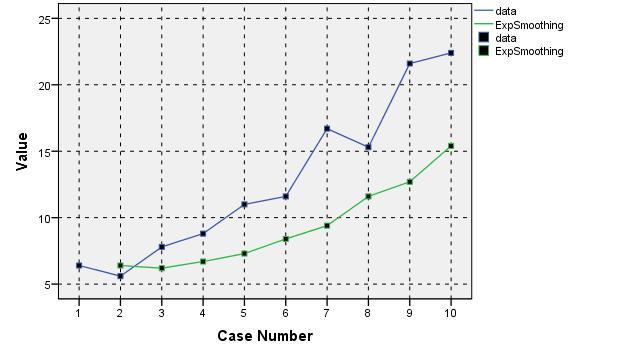
\includegraphics[width=1.00\textwidth]{time-series/time-series-61.jpg}
  \caption{Exponential smoothing for a trend}
  \label{fig:time-series-61}
\end{figure}

Therefore, we add an extra constant to bridge this gap:

\begin{definition}[Holt forcasting or double exponential smoothing]
\begin{eqnarray}
  X_{t} = \alpha x_{t} + (1-\alpha)(X_{t-1} + b_{t-1}) & 0 \leq \alpha \leq 1 \\
  b_{t} = \beta(X_{t}-X_{t-1}) + (1-\beta)b_{t-1} & 0 \leq \beta \leq 1 
\label{eq:doubleSmoothing}
\end{eqnarray}
\end{definition}

\subsection{Initial value}

As with basic exponential smoothing, there are different methods for selecting the initial values of $X_{t}$ and $b_{t}$:

\begin{itemize}
	\item $X_{1} = x_{1}$
	\item $b_{1} = x_{2} - x_{1}$
	\item $b_{1} = \frac{1}{3}\left[ (x_{2} - x_{1}) + (x_{1} - x_{2}) + (x_{4} - x_{3}) \right]$
	\item $b_{1} = \frac{x_{n} - x_{1}}{n-1}$
\end{itemize}

\subsubsection{Prediction}

Making a prediction when using double exponential smoothing is slightly different ($F_{t+1}$ is used as prediction for time $T+1$):

\[ F_{t+1} = X_{t} + b_{t} \]
or
\[ F_{t+m} = X_{t} + m b_{t} \]

If we now draw a plot with basic exponential smoothing ($\alpha = 0.977$) and double exponential smoothing ($\alpha = 0.3623, \beta = 1.0, X_{1} = x_{1} = 6.4$ and $b_{1} = \frac{1}{3}\left[ (x_{2} - x_{1}) + (x_{1} - x_{2}) + (x_{4} - x_{3}) \right] = 0.8$) we obtain the values of Table \ref{tab:doubleSingle} and Figure \ref{fig:time-series-71}:

\begin{table}
  \centering
  \begin{tabular}{|llll|}
    \hline
    Data & Basic exponential smoothing $X_{t}$ & Double exponential smoothing $X_{t}$ & $F_{t}$ \\
    6.4  & ~                      & 6.4              & ~                             \\
    5.6  & 6.4                    & 6.6              & 7.2                           \\
    7.8  & 5.6                    & 7.2              & 6.8                           \\
    8.8  & 6.7                    & 8.1              & 7.8                           \\
    11.0 & 8.8                    & 9.8              & 9.1                           \\
    11.6 & 10.9                   & 11.5             & 11.4                          \\
    16.7 & 11.6                   & 14.5             & 13.2                          \\
    15.3 & 16.6                   & 16.7             & 17.4                          \\
    21.6 & 15.3                   & 19.9             & 18.9                          \\
    22.4 & 21.5                   & 22.8             & 23.1                          \\ \hline
  \end{tabular}
  \caption{Table with basic and double exponential smoothing}
  \label{tab:doubleSingle}
\end{table}

\begin{figure}
	\centering
		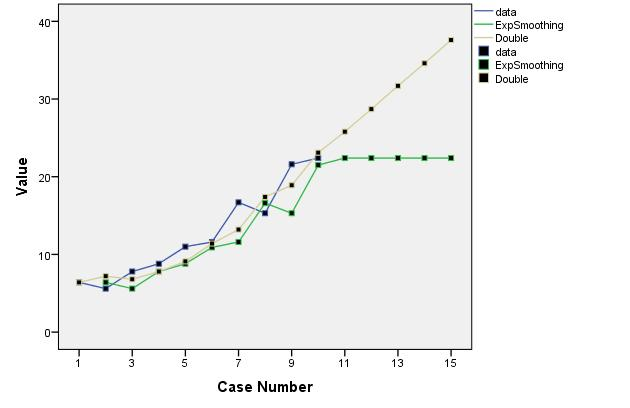
\includegraphics[width=1.00\textwidth]{time-series/time-series-71.jpg}
	\caption{Basic and double exponential smoothing}
	\label{fig:time-series-71}
\end{figure}

The procedure to solve this in R is similar to the procedure for basic exponential smoothing, except that the parameter $\beta$ should not be set to NULL. Creating the correlogram, applying the Ljung–Box test and testing the normality of the errors is done in a similar way.

\subsection{Triple exponential smoothing}

In many time series you will see that certain patterns recur. For example, take the daily turnover of a bakery: the turnover will be different every day, but if you look at it over a long period of time, you will probably see a similar pattern every week (with a top turnover on Sunday, for example).

This type of time series can be approximated by using the Holt-Winter method, or triple exponential smoothing.

\begin{eqnarray}
  X_{t} = \alpha \frac{x_{t}}{c_{t-L}} + (1-\alpha) (X_{t-1} + b_{t-1}) & \textnormal{Smoothing}\\
  b_{t} = \beta (X_{t} - X_{t-1}) + (1-\beta)b_{t-1} & \textnormal{Trend smoothing} \\
  c_{t} = \gamma \frac{x_{t}}{X_{t}} + (1-\gamma)c_{t-L} & \textnormal{Seasonal smoothing} \\
  F_{t+m} = (X_{t} + mb_{t})c_{t-L+m \mod L}  & \textnormal{Prediction}
  \label{eq:HoltWinters}
\end{eqnarray}
 with
\begin{itemize}
	\item $x_{t}$ the observation at time $t$
	\item $X_{t}$ the smoothed observation at time $t$
	\item $b_{t}$ the trend factor at time $t$
	\item $c_{t}$ the seasonal index at time $t$
	\item $F_{t}$ the prediction at time $t$
	\item $L$ the period (e.g. of the seasons)
\end{itemize}

$\alpha, \beta en \gamma$ are constants that need to be estimated.
The procedure to solve this in R is similar to the procedure for basic exponential smoothing. Creating the correlogram, applying the Ljung–Box test and testing the normality of the errors is done in a similar way.

\section{Exercises}
\label{sec:time-series-exercises}

\begin{exercise}
  The file \emph{Budget.csv} contains the turnover, advertising budget and GNP (Dutch: BNP) of a medium sized compay per quarter between 1981 and 2005. Add another column yourself that contains an ascending number for each quarter.
  
  \begin{enumerate}
    \item Calculate the basic (or simple) moving average over periods 4 and 12 of this data. Use the SMA method for this. Plot a line graph for $X$, $SMA(4)$ and $SMA(12)$.
    \item Which previously covered technique (from the section on descriptive statistics) is also suitable for making predictions about the values of $X$? Do so using the appropriate function and plot the results in the graph.
    \item Use the \emph{forecast} method to make predictions for the next 10 periods using each of the previous methods (moving average 4, 10 and regression). Also plot the results on the graph.
    \item Is the use of one of these techniques interesting to make predictions for this data?
    \item Create a time series of the data using the method \emph{ts}. Use the \emph{decompose} method to divide the time series and get an idea of the trend and the seasonal fluctuation.
    \item Calculate the exponential moving average (\emph{EMA}) using the method \emph{HoltWinters}. Make another prediction for 20 periods using the \emph{forecast} method. For the initial values, use $s_1 = x_1$ and the value generated by R for $\alpha$. Plot the result in a new graph, together with $X$.
    \item Do the same for $\alpha=0.1$.
    \item What do the predictions look like?
    \item Do the same using \emph{double} exponential smoothing. For the initial values, use $s_1 = x_1$ and $b_1 = \frac{x_n - x_1}{n - 1}$, $\alpha =  0.05$ and $\beta = 0.2$. Plot the result on the graph.
    \item Use double exponential smoothing to calculate predictions for 20 periods. Plot the values on the graph. Is this technique better or worse than the previous one for this dataset?
    \item Experiment with the value $\alpha$ and $\beta$ and look at the result, for both basic and double exponential smoothing.
    \item Use the \emph{HoltWinters} method without trend. In other words, use $\beta=0$. For the initial values, use $\alpha =  0.05$ and $\gamma = 0.9$. Plot the result on the graph.
    \item Again, calculate predictions for 20 periods. Plot the values on the graph. Is this technique better or worse than the previous one for this dataset?
    \item Experiment with the values of $\alpha$, $\beta$ and $\gamma$ and look at the result.
    \item Use the \emph{HoltWinters} method with the values generated by R, but again without using a trend ($\beta=0$). Plot the result on the graph.
    \item Again, calculate predictions for 20 periods but this time by using the function \emph{predict}. Plot the values on the graph. Is this technique better or worse than the previous one for this dataset?
  \end{enumerate}	
  \end{exercise}
  
  \begin{exercise}
  The file \emph{Passagiers2.csv} contains the number of passengers on an airline between January 1949 and December 1960.
  \begin{enumerate}
    \item Calculate the basic (or simple) moving average over periods 4 and 12 of this data. Use the \emph{MA} method for this. Plot a line graph for $X$, $MA(4)$ and $MA(12)$.
    \item Which previously covered technique (from the section on descriptive statistics) is also suitable for making predictions about the values of $X$? Do so using the appropriate function and plot the results in the graph.
    \item Use the \emph{forecast} method to make predictions for the next 10 periods using each of the previous methods (moving average 4, 12 and regression). Also plot the results on the graph. What is your conclusion?
    \item Is the use of one of these techniques interesting for making predictions for this data?
    \item Use the method \emph{decompose} to subdivide the time series and get an idea of the trend and the seasonal fluctuation.
    \item Calculate the exponential moving average (\emph{EMA}) using the \emph{ses} method with $\alpha=0.2$. Make another prediction using the \emph{forecast} method for 20 periods. Plot the result in a new graph, together with $X$.
    \item Do the same for $\alpha=0.6$ and $\alpha=0.89$.
    \item What to the predictions look like now?
    \item Do the same using \emph{double} exponential smoothing. Use the \emph{holt} method for this, with $\alpha =  0.8$ and $\beta = 0.2$. Plot the result on the graph.
    \item Use double exponential smoothing to calculate predictions for 20 periods. Plot the values on the graph. Is this technique better or worse than the previous one for this dataset?
    \item Add the option $exponential=TRUE$ to the method. Plot the result. What is the difference?
    \item Use the \emph{hw} method with the values generated by R. Plot the result on the graph.
    \item Again, calculate a few predictions using the method \emph{predict}. Plot the values on the graph. Is this technique better or worse than the previous one for this dataset?
    \item Experiment with the values for $\alpha$, $\beta$ and $\gamma$ and look at the result.
  \end{enumerate}
  
  \end{exercise}
